\chapter{Аналитический раздел}

Одной из главных причин низкой скорости обработки запросов является работа с базой данных (БД), которая не оптимизирована: нерациональные запросы, некорректное использование индексов, неоптимальные значения параметров конфигурации. 

Оптимизация производительности сводится к следующим задачам: 
\begin{enumerate}
\item корректировка параметров СУБД;
\item денормализация данных (при необходимости);
\item выявление медленных запросов, их анализ;
\item корректировка запросов;
\item создание индексов.
\end{enumerate}

Основным приемом увеличения производительности выполнения запросов к базе данных является индексирование. Индексы представляют собой структуры, которые помогают MySQL эффективно извлекать данные. Они критичны для достижения хорошей производительности, но многие часто забывают о них или плохо понимают их смысл, поэтому индексирование является главной причиной проблем с производительностью в реальных условиях. \cite{zaitsev}

Индексы увеличивают производительность путем оптимизации обращений к дисковой памяти.

Индексы следует создавать по мере обнаружения медленных запросов. В этом поможет \textit{slow log} в MySQL. Запросы, которые выполняются более 1 секунды, являются первыми кандидатами на оптимизацию. \cite{ruhighload-mysql-indexes} Конечно, говорить о том, сколько секунд считать медленным запросом зависит от конкретной задачи. В основном такие запросы используют JOIN оператор для соединения двух и более таблиц.

Задачу выбора индекса для конкретного sql запроса на БД, заполненной реальными данными, решают СУБД. На текущий момент даже сами БД не справляются с этой задачей. Но если абстрагироваться от реальных данных, которыми заполнена СУБД и статистики запросов, то зная правила работы СУБД с индексами можно сделать предположения, какие индексы могла бы использовать СУБД. В данной работе предлагаются алгоритмы, которые по заданному sql запросу вернут список индексов, которые могли бы использоваться СУБД при выполнении этого запроса. Дальше, администратор БД примет решение, какой именно индекс построить из предложенного списка.

\section{Структура индексов в MySQL InnoDB}

В СУБД MySQL (InnoDB) используются Btree индексы, основанные на структуре данных B+tree Рисунок \ref{img:btree-structure}.

\begin{figure}[H]
  \centering
  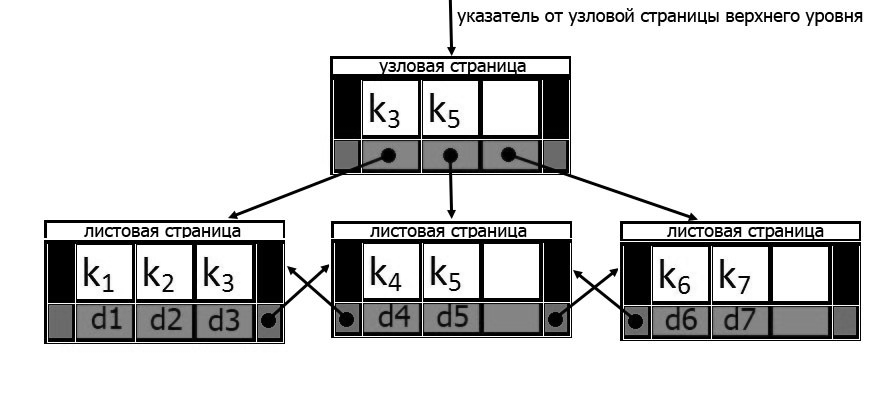
\includegraphics[scale=0.5]{btree.png}
  \caption{Структура данных B+tree.}
  \label{img:btree-structure}
\end{figure}

Где
$k_i$ - ключи ($k_i < k_i + 1$),
$d_i$ - данные.

Сложность поиска в линейной структуре данных $O(N)$, а в B+tree - $log(K)+N_k$, где $k$ — количество уровней, а $N_k$ — количество элементов в узле. Поэтому индексы, использующие структуру данных B+tree, эффективны для поиска данных. Для оптимизации поиска по диапазону в листовых страницах есть указатели на следующую и предыдущую листовую страницу.

В InnoDB данные хранятся в структуре B+tree, где в узловых страницах хранятся первичные ключи, а в листовых страницах хранятся данные. Такое дерево называется \textbf{кластерным индексом}. Над таблицей можно построить только один кластерный индекс, поскольку невозможно хранить одну и ту же запись одновременно в двух местах. Однако часть записи можно хранить в нескольких местах, что будет использоваться в покрывающих индексах, являющимися вторичными индексами.

Для оптимизации конкретных запросов используются \textbf{вторичные индексы} (далее просто индексы). В узловых страницах индексов хранятся поля, по которым создан этот индекс, а в листовых страницах хранится значение первичного ключа. Для каждой таблицы в одном запросе используется только один индекс. При использовании в запросах индекса, сначала будет найдено значение первичного ключа, затем по этому значению будут найдены данные в кластерном индексе.

\subsection{Индексы для простых запросов}

Чтобы построить индексы для простых запросов (т.е. без соединения таблиц) необходимо воспользоваться простыми правилами.

%Скопировать из дока


\subsection{Индексы для сложных запросов}

Построение индексов для запроса с соединением таблиц часто вызывает сложности, так как требует от разработчика знания тонкостей работы СУБД при соединении таблиц, и тонкостей работы с индексами. Раньше не предлагалось общего алгоритма построения индексов на запросы с соединением таблиц. В данной работе предлагается такой алгоритм, который может иметь программную реализацию.